\subsection{Light\-Curve  Class Reference}
\label{class_lightcurve}\index{LightCurve@{Light\-Curve}}
The same Fiducial\-Star monitored many nights. 


{\tt \#include $<$lightcurve.h$>$}

Inheritance diagram for Light\-Curve::\begin{figure}[H]
\begin{center}
\leavevmode
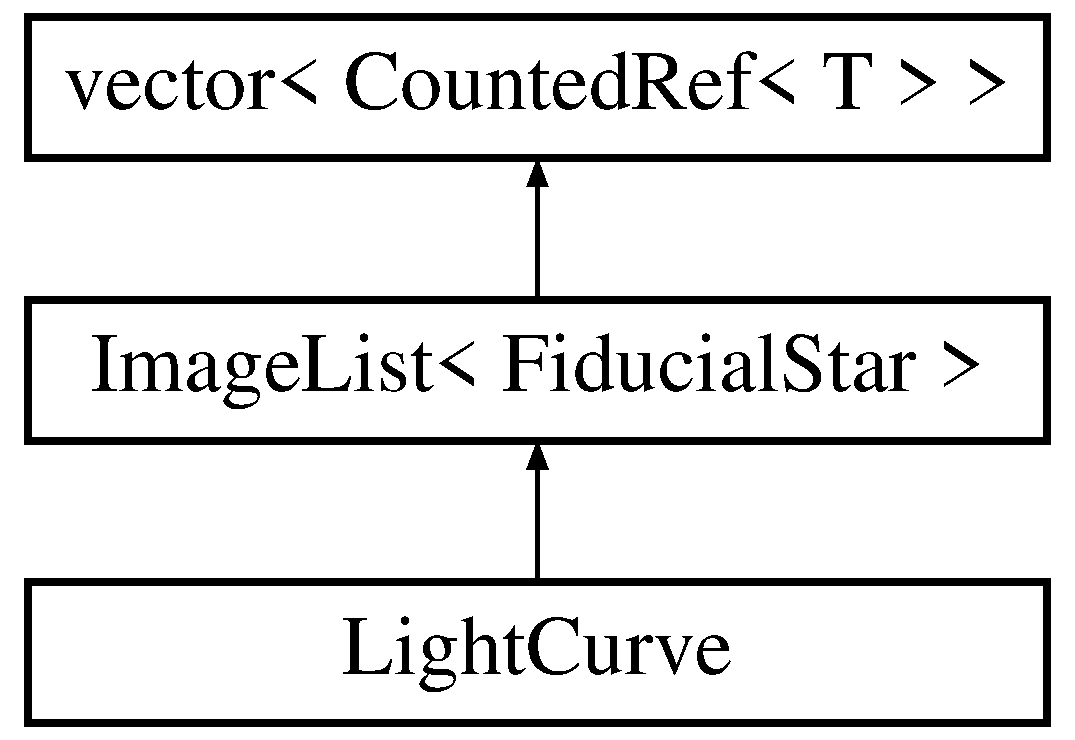
\includegraphics[height=3cm]{class_lightcurve}
\end{center}
\end{figure}
\subsubsection*{Public Methods}
\begin{CompactItemize}
\item 
\index{LightCurve@{LightCurve}!LightCurve@{Light\-Curve}}\index{LightCurve@{LightCurve}!LightCurve@{Light\-Curve}}
{\bf Light\-Curve} (const Night\-List \&All\-Nights, const Phot\-Star \&One\-Star)\label{class_lightcurve_a0}

\item 
\index{LightCurve@{LightCurve}!LightCurve@{Light\-Curve}}\index{LightCurve@{LightCurve}!LightCurve@{Light\-Curve}}
{\bf Light\-Curve} (istream \&Stream)\label{class_lightcurve_a1}

\item 
\index{LightCurve@{LightCurve}!LightCurve@{Light\-Curve}}\index{LightCurve@{LightCurve}!LightCurve@{Light\-Curve}}
{\bf Light\-Curve} ()\label{class_lightcurve_a2}

\item 
\index{AveragePosition@{AveragePosition}!LightCurve@{Light\-Curve}}\index{LightCurve@{LightCurve}!AveragePosition@{Average\-Position}}
void {\bf Average\-Position} ()\label{class_lightcurve_a3}

\begin{CompactList}\small\item\em take the weighted mean of all positions.\item\end{CompactList}\item 
\index{RelativeFluxes@{RelativeFluxes}!LightCurve@{Light\-Curve}}\index{LightCurve@{LightCurve}!RelativeFluxes@{Relative\-Fluxes}}
void {\bf Relative\-Fluxes} ()\label{class_lightcurve_a4}

\begin{CompactList}\small\item\em compute the relative fluxes according to the night photometric ratios.\item\end{CompactList}\item 
\index{AbsoluteFluxes@{AbsoluteFluxes}!LightCurve@{Light\-Curve}}\index{LightCurve@{LightCurve}!AbsoluteFluxes@{Absolute\-Fluxes}}
void {\bf Absolute\-Fluxes} ()\label{class_lightcurve_a5}

\begin{CompactList}\small\item\em compute the absolute calibrated fluxes.\item\end{CompactList}\item 
\index{dump@{dump}!LightCurve@{Light\-Curve}}\index{LightCurve@{LightCurve}!dump@{dump}}
void {\bf dump} (ostream \&Stream=cout) const\label{class_lightcurve_a6}

\item 
\index{write_header@{write\_\-header}!LightCurve@{Light\-Curve}}\index{LightCurve@{LightCurve}!write_header@{write\_\-header}}
void {\bf write\_\-header} (ostream \&Stream) const\label{class_lightcurve_a7}

\item 
\index{write@{write}!LightCurve@{Light\-Curve}}\index{LightCurve@{LightCurve}!write@{write}}
void {\bf write} (ostream \&Stream) const\label{class_lightcurve_a8}

\item 
\index{write@{write}!LightCurve@{Light\-Curve}}\index{LightCurve@{LightCurve}!write@{write}}
void {\bf write} (const string \&File\-Name) const\label{class_lightcurve_a9}

\item 
\index{read@{read}!LightCurve@{Light\-Curve}}\index{LightCurve@{LightCurve}!read@{read}}
void {\bf read} (istream \&Stream)\label{class_lightcurve_a10}

\end{CompactItemize}
\subsubsection*{Public Attributes}
\begin{CompactItemize}
\item 
\index{refstar@{refstar}!LightCurve@{Light\-Curve}}\index{LightCurve@{LightCurve}!refstar@{refstar}}
Phot\-Star {\bf refstar}\label{class_lightcurve_m0}

\item 
\index{IsStandard@{IsStandard}!LightCurve@{Light\-Curve}}\index{LightCurve@{LightCurve}!IsStandard@{Is\-Standard}}
bool {\bf Is\-Standard}\label{class_lightcurve_m1}

\begin{CompactList}\small\item\em returns true if the Fiducial\-Star is a standard star.\item\end{CompactList}\item 
\index{FidName@{FidName}!LightCurve@{Light\-Curve}}\index{LightCurve@{LightCurve}!FidName@{Fid\-Name}}
string {\bf Fid\-Name}\label{class_lightcurve_m2}

\begin{CompactList}\small\item\em name of the star, useful for bookeeping.\item\end{CompactList}\end{CompactItemize}
\subsubsection*{Friends}
\begin{CompactItemize}
\item 
\index{ByIncreasingFlux@{ByIncreasingFlux}!LightCurve@{Light\-Curve}}\index{LightCurve@{LightCurve}!ByIncreasingFlux@{By\-Increasing\-Flux}}
bool {\bf By\-Increasing\-Flux} (const Fiducial\-Star $\ast$one, const Fiducial\-Star $\ast$two)\label{class_lightcurve_l0}

\begin{CompactList}\small\item\em sorts by increasing fluxes.\item\end{CompactList}\item 
\index{ByIncreasingSignalToNoise@{ByIncreasingSignalToNoise}!LightCurve@{Light\-Curve}}\index{LightCurve@{LightCurve}!ByIncreasingSignalToNoise@{By\-Increasing\-Signal\-To\-Noise}}
bool {\bf By\-Increasing\-Signal\-To\-Noise} (const Fiducial\-Star $\ast$one, const Fiducial\-Star $\ast$two)\label{class_lightcurve_l1}

\begin{CompactList}\small\item\em sorts by increasing signal to noise.\item\end{CompactList}\end{CompactItemize}


\subsubsection{Detailed Description}
The same Fiducial\-Star monitored many nights.



The documentation for this class was generated from the following file:\begin{CompactItemize}
\item 
{\bf lightcurve.h}\end{CompactItemize}
